% Тут используется класс, установленный на сервере Papeeria. На случай, если
% текст понадобится редактировать где-то в другом месте, рядом лежит файл matmex-diploma-custom.cls
% который в момент своего создания был идентичен классу, установленному на сервере.
% Для того, чтобы им воспользоваться, замените matmex-diploma на matmex-diploma-custom
% Если вы работаете исключительно в Papeeria то мы настоятельно рекомендуем пользоваться
% классом matmex-diploma, поскольку он будет автоматически обновляться по мере внесения корректив
%

% По умолчанию используется шрифт 14 размера. Если нужен 12-й шрифт, уберите опцию [14pt]
\documentclass[14pt]{matmex-diploma}
%\documentclass[14pt]{matmex-diploma-custom}
\usepackage{verbatim}
\usepackage{verbatim}
\usepackage{float}
\usepackage{caption}
\usepackage{subcaption}
\usepackage{graphicx}
\usepackage{minted}
\usepackage{verbments}
\usepackage{array}
\usepackage{tikz}
\usepackage{pgfplots}
\pgfplotsset{compat=1.9}
\renewcommand\listingscaption{Листинг}
\begin{document}
% Год, город, название университета и факультета предопределены,
% но можно и поменять.
% Если англоязычная титульная страница не нужна, то ее можно просто удалить.
\filltitle{ru}{
    chair              = {Кафедра Системного программирования},
    title              = {Использование символьных конечных преобразователей для лексического анализа динамически формируемого кода},
    % Здесь указывается тип работы. Возможные значения:
    %   coursework - Курсовая работа
    %   diploma - Диплом специалиста
    %   master - Диплом магистра
    %   bachelor - Диплом бакалавра
    type               = {coursework},
    position           = {студента},
    group              = 371,
    author             = {Гумин Егор Дмитриевич},
    supervisorPosition = {ст. пр.},
    supervisor         = {Григорьев  С.\,В.},
    reviewerPosition   = {ст. преп.},
    reviewer           = {Привалов А.\,И.},
    chairHeadPosition  = {д.\,ф.-м.\,н., профессор},
    chairHead          = {Хунта К.\,Х.},
%   university         = {Санкт-Петербургский Государственный Университет},
%   faculty            = {Математико-механический факультет},
%   city               = {Санкт-Петербург},
%   year               = {2013}
}





\maketitle
\tableofcontents
% У введения нет номера главы
\section*{Введение}
Существует подход к написанию программного кода, при котором код на одном языке программирования формируется программой на другом языке с помощью строковых операций, циклов и условных операторов. Такой код называется динамически формируемым. В качестве примера можно рассмотреть генерацию html-страниц в языке Javascript или формирования SQL-запросов в C\# с помощью строковых операций. На листинге~\ref{lst:example1} представлен пример динамически формируемого кода.

\fvset{frame=lines,framesep=5pt}
\begin{listing}[H]
    \begin{pyglist}[language=csharp,numbers=left,numbersep=5pt]
 private void Go(int cond){
   string columnName = cond > 3 ? "X" : (cond < 0 ? "Y" : "Z");
   string queryString = 
       "SELECT name" + columnName + " FROM table";
   Program.ExecuteImmediate(queryString);}
    \end{pyglist}
\caption{Пример динамически формируемого кода}
\label{lst:example1}
\end{listing}

Этот подход был достаточно распространен, поэтому существует большое множество программ, использующих его. Кроме того, иногда возникает необходимость написания такого кода (например, в случаях, когда ограничения по производительности не позволяют использовать ORM). Статический анализ такого кода, например, подсветка синтаксиса и диагностика ошибок, позволил бы существенно упростить его написание и поддержку.

Существует ряд инструментов~\cite{Alvor, JSA, PHPSA} (подробно рассмотрены в работе ~\cite{polubelova}), позволяющих проводить статический анализ динамически формируемого кода. Однако эти инструменты обладают такими недостатками, как слабая расширяемость, ограниченная функциональность, применимость только к конкретным языкам. Для решения этих проблем~\cite{GrigorievPhd} в рамках проекта YaccConstructor~\cite{YCUrl, articleYC}, который посвящен исследованиям в области лексического и синтаксического анализа, реализована платформа для работы со встроенными языками. Модульность платформы позволяет легко добавлять дополнительную функциональность и поддержку новых языков. статический анализ динамического кода производится в несколько шагов: 
\begin{enumerate}
\item построение регулярной аппроксимации сверху множества значений динамически формируемого выражения;
\item лексический анализ;
\item синтаксический анализ;
\item семантический анализ.
\end{enumerate}

% * <colored.lime@gmail.com> 14:34:52 25 May 2016 UTC+0300:
% fix
Но механизм лексического анализа~\cite{polubelova} в проекте YaccConstructor, использующий композицию конечных преобразователей, обладает недостаточной производительностью. Вероятная причина этой проблемы - разрастание конечных преобразователей на больших алфавитах, так как обработка большого количества дуг занимает много времени. Возможное решение - применение символьных конечных преобразователей~\cite{st}, с помощью которых можно представить структуры данных более компактно. 
На данный момент единственной библиотекой для работы с символьными конечными преобразователями в рамках платформы .NET является библиотека Microsoft.Automata~\cite{MSAUrl}, которая активно поддерживается сообществом Microsoft Research, именно поэтому она и является предметом изучения.
В рамках данной работы исследован вопрос о возможности увеличения производительности лексического анализа с помощью использования символьных конечных преобразователей из библиотеки Microsoft.Automata.

% * <colored.lime@gmail.com> 14:35:11 25 May 2016 UTC+0300:
% fix\


\section{Постановка задачи}
Целью данной работы является исследование применимости символьных конечных преобразователей для лексического анализа. Для ее достижения поставлены следующие задачи.
\begin{itemize}
    \item Изучить возможности библиотеки Microsoft.Automata.
\item Провести сравнение производительности алгоритма операции композиции над символьными конечными преобразователями в библиотеке Microsoft.Automata с производительностью операции композиции над конечными преобразователями в исследовательском проекте YaccConstructor.
\item На основании полученных результатов сделать выводы о применимости библиотеки Microsoft.Automata для лексического анализа в проекте YaccConstructor.
  \end{itemize}

\section{Обзор}
В данной главе определены основные понятия и проведен обзор основных применяемых формализмов, инструментов и технологий.

\subsection{Конечные преобразователи}
\textbf{Конечный преобразователь~\cite{FST}} (Finite State Transducer) --- формализм, напоминающий конечный автомат, который при переходе из состояния в состояние пишет символ в выходной поток.
Конечный преобразователь можно задать шестеркой элементов: 
$\langle Q, \Sigma, \Delta, q_0, F, E \rangle$, где

\begin{itemize}
\item $Q$ --- множество состояний, 
\item $\Sigma$ --- входной алфавит, 
\item $\Delta$ --- выходной алфавит, 
\item $q_0 \in Q$ --- начальное состояние, 
\item $F \subseteq Q$ --- набор конечных состояний, 
\item $E \subseteq Q \times (\Sigma \cup \{\varepsilon\}) \times (\Delta \cup \{\varepsilon\})  \times Q$ --- набор переходов. 
\end{itemize}

Важнейшей для лексического анализа операцией над конечными преобразователями является операция композиции. Результат композиции двух конечных преобразователей — конечный преобразователь, работающий так, будто входной поток первого переправили во входной поток второго. Формальное определение дано ниже.

\textbf{Композицией} конечных преобразователей 
$T_1~=~\langle Q_1, \Sigma_1, \Delta_1, q_{0_{1}}, F_1, E_1 \rangle$ и $T_2~=~\langle Q_2, \Sigma_2, \Delta_2, q_{0_{2}}, F_2, E_2 \rangle$ является конечный преобразователь  $T =\langle Q_1  \times Q_2, \Sigma_1, \Delta_2, \langle q_{0_{1}}, q_{0_{2}} \rangle, F_1 \times F_2, E \cup E_{\varepsilon} \cup E_{i,\varepsilon} \cup E_{o,\varepsilon} \rangle$, где 

\begin{itemize}
\item $E = \{ \langle \langle p, q \rangle, a, b, \langle p', q' \rangle \rangle\ | \exists c \in \Delta_1 \cap \Sigma_2 : \langle p, a, c, p' \rangle \in E_1 \wedge \langle q, c, b, q' \rangle \in E_2\}$
\item $E_{\varepsilon} = \{ \langle \langle p, q \rangle, a, b, \langle p', q' \rangle \rangle\ | \langle p, a, {\varepsilon}, p' \rangle \in E_1 \wedge \langle q, {\varepsilon}, b, q' \rangle \in E_2\}$
\item $E_{i, \varepsilon} = \{ \langle \langle p, q \rangle, {\varepsilon}, a, \langle p, q' \rangle \rangle\ | \langle q, {\varepsilon}, a, q' \rangle \in E_2 \wedge p \in Q_1 \} $
\item $E_{o, \varepsilon} = \{ \langle \langle p, q \rangle,  a, {\varepsilon}, \langle p', q \rangle \rangle\ | \langle p, a, {\varepsilon}, p' \rangle \in E_1 \wedge q \in Q_2 \}. $
\end{itemize}

На рисунках ~\ref{compose1}-~\ref{compose3} представлен пример композиции конечных преобразователей. Результатом композиции конечного преобразователя $T_1$ с рисунка~\ref{compose1} с конечным преобразователем $T_2$ с рисунка~\ref{compose2} будет конечный преобразователь с рисунка~\ref{compose3}.

\begin{figure}[h!]
        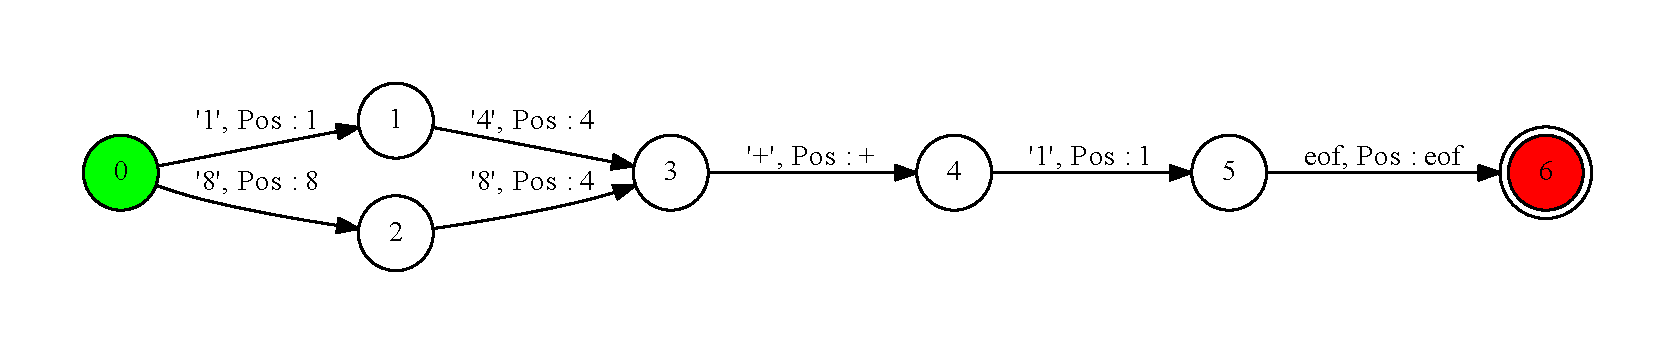
\includegraphics[width=\linewidth]{../pictures/example_.pdf}
        \caption{Конечный преобразователь $T_1$}
        \label{compose1} 
\end{figure}

\begin{figure}[h!]
        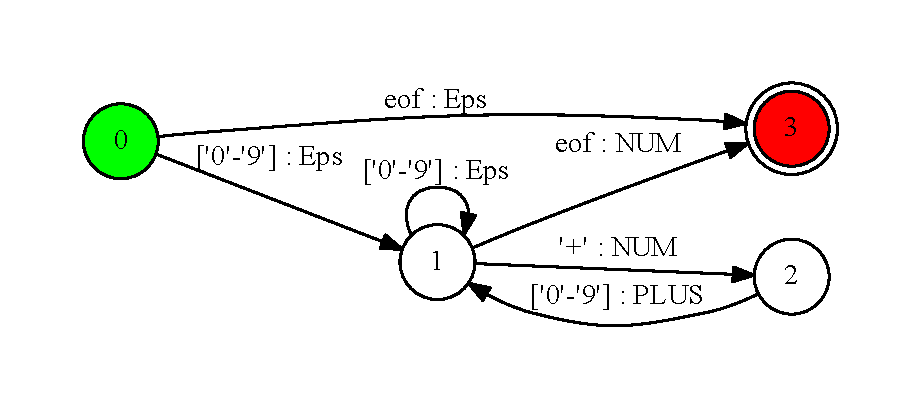
\includegraphics[width=13cm]{../pictures/lexer_.pdf}
        \caption{Конечный преобразователь $T_2$}
        \label{compose2} 
\end{figure}

\begin{figure}[h!]
        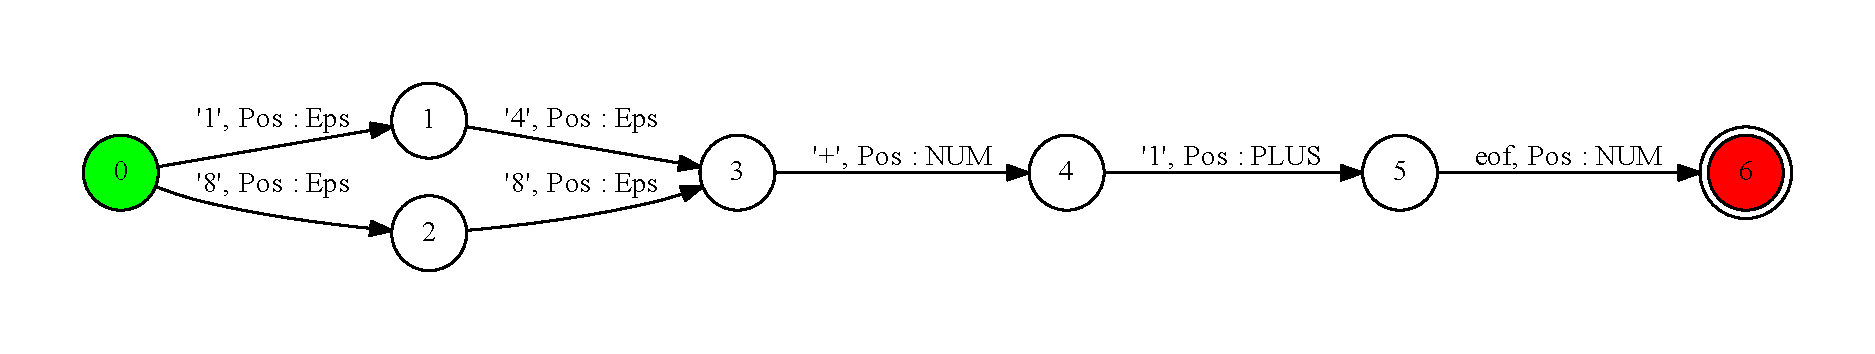
\includegraphics[width=\linewidth]{../pictures/res_.pdf}
        \caption{Результат композиции конечных преобразователей $T_1$ и $T_2$}
        \label{compose3} 
\end{figure}

\subsection{Символьные конечные преобразователи}
При разработке лексических анализаторов часто возникает ситуация, когда из одного состояния в другое необходимы переходы сразу по нескольким символам. Преобразователи часто реализовывают как некоторые графы, и каждый переход представляется как дуга в этом графе. Соответственно, при разработке лексических анализаторов часто приходится добавлять много дублирующих ребер, например, если необходимо, по любой цифре перейти из состояния А в состояние В, нужно добавить 10 дуг (рисунок~\ref{fig:numfst}). Чем больше ребер в графе, тем больше расход памяти и ниже производительность.

Для борьбы с этой проблемой был предложен символьный конечный преобразователь (Symbolic Transducer) --- конечный преобразователь,  каждому переходу которого можно сопоставить не один символ, а формулу (например, регулярное выражение). Таким образом, в приведенном выше примере вместо десяти дуг будет одна дуга, которой соответствует регулярное выражение (рисунок~\ref{fig:numst}), описывающее цифры. Такие преобразователи получаются гораздо более компактными. 

\begin{figure}[h!]
    \begin{center}
        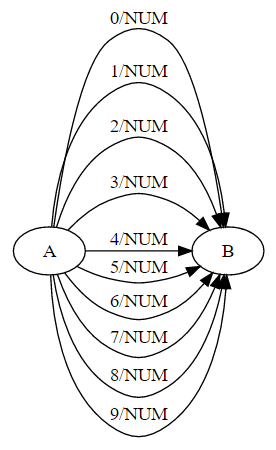
\includegraphics[width=\linewidth/3]{pictures/NumFST.png}
        \caption{Пример конечного преобразователя}
        \label{fig:numfst} 
    \end{center}
\end{figure}

\begin{figure}[h!]
    \begin{center}
        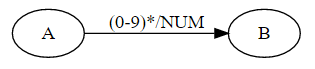
\includegraphics[width=\linewidth/2]{pictures/NumST.png}
        \caption{Символьный конечный преобразователь, эквивалентный конечному преобразователю на рис. 4}
        \label{fig:numst} 
    \end{center}
\end{figure}

\textbf{Символьный конечный преобразователь} можно задать шестеркой элементов: 
$\langle Q, \Sigma, \Delta, q_0, F, E \rangle$, где

\begin{itemize}
\item $Q$ --- множество состояний, 
\item $\Sigma$ --- входной алфавит, 
\item $\Delta$ --- выходной алфавит, 
\item $q_0 \in Q$ --- начальное состояние, 
\item $F \subseteq Q$ --- набор конечных состояний, 
\item $E \subseteq Q \times (R(\Sigma) \cup \{\varepsilon\}) \times (\Delta \cup \{\varepsilon\})  \times Q$ --- набор переходов, $R(X)$ --- некоторая формула (в нашем случае --- регулярное выражение) над множеством $X$.
\end{itemize}

\subsection{Лексический анализ}
Основной задачей лексического анализа является выделение лексем во входном потоке с сохранением их привязки к исходному коду. При лексическом анализе статического кода поток символов линеен, но в случае анализа встроенного кода он линейным не является. Поэтому применяется следующий подход.

\begin{enumerate}
\item В некоторой точке программы по множеству значений строкового выражения строится конечный автомат $M$, аппроксимирующий его сверху.
\item По конечному автомату $M$ строится конечный преобразователь.
\item Производится композиция конечного преобразователя $M$ с конечным преобразователем, являющимся лексическим анализатором языка, на котором написано строковое выражение.
\item По результирующему преобразователю строится конечный автомат над лексемами, который и является токенизированным входом.
\end{enumerate}

Сложность операции композиции зависит от количества ребер, символьные преобразователи обычно содержат меньшее их количество, чем эквивалентные конечные преобразователи, что позволяет увеличить производительность композиции.

\subsection{Библиотека Microsoft.Automata}
Microsoft.Automata --- .NET-библиотека, содержащая реализации конечных автоматов, конечных преобразователей, операции над ними и средства их анализа. Библиотека состоит из следующих модулей.
\begin{itemize}
\item Automata --- основной модуль с реализацией автоматов и преобразователей, содержащий в себе такие элементы, как:
    \begin{itemize}
    \item синтаксические анализаторы грамматик для построения по ним автоматов;
    \item синтаксические анализаторы регулярных выражений, которые используются при построении преобразователей;
    \item различные структуры данных, например, BDD;
    \item символьные автоматы и операции над ними;
    \item символьные преобразователи и операции над ними Z3~\cite{STcompose}. 
    \end{itemize}
\item Automata.Z3 --- модуль, обеспечивающий интеграцию реализованных формализмов с SMT-решателем Z3~\cite{Z3Url, articleZ3}.
\item Bek --- модуль, позволяющий работать с преобразователями и автоматами, используя язык Bek Z3~\cite{BekUrl, BekArticle}. Язык Bek - предметно-ориентированный язык для написания и анализа конечных преобразователей, работающих со строками, который является аналогом регулярных выражений для автоматов. Программы на Bek позволяют ответить на вопросы <<Выводят ли две программы одну и ту же строку>>, <<Может ли эта программа вывести некоторую строку?>>, <<Что будет, если выполнить композицию программ?>>.

На листинге~\ref{lst1} приведен пример программы на языке Bek. Программа проходит по строке, используя переменную c, чтобы итерироваться по символам и булеву переменную b, чтобы отслеживать, был ли предыдущий символ экранирующим и добавляет экранирующий символ перед одинарными или двойными кавычками, если он пропущен. 

\fvset{frame=lines,framesep=5pt}
\begin{listing}[H]
    \begin{pyglist}[language=csharp,numbers=left,numbersep=5pt]
program sanitize(t);
    string s; 
    s := iter(c in t){b := false;}{
            case (!(b) && ((c == '\'') || (c == '\"'))) :
                b := false;
                yield ('\\');
                yield (c);
            case (c == '\\') :
                b := !(b);
                yield (c);
            case (true) :
                b := false;
                yield (c);
            };
    return s;
    \end{pyglist}
\caption{Пример программы на языке Bek}
\label{lst1}
\end{listing}
\end{itemize}

\section{Окружение для тестирования и экспериментальное исследование}
В данной главе описывается реализация окружения для тестирования производительности операции композиции на символьных конечных преобразователях в библиотеке Microsoft.Automata и конечных преобразователях в YaccConstructor. Также приведено описание процесса тестирования и сделаны выводы о применимости символьных преобразователей из библиотеки Microsoft.Automata в исследовательском проекте YaccConstructor.

При изучении возможностей библиотеки, проведенном в рамках обзора, было установлено, что полная интеграция проекта YaccConstructor  и библиотеки Microsoft.Automata затруднительна. По этой причине для оценки производительности библиотеки Microsoft.Automata было необходимо создать окружение для тестирования, обеспечивающее возможность генерации тестов по одинаковым данным для разнородных сред: инструмента YaccConstructor и библиотеки Microsoft.Automata.

\subsection{Окружение для тестирования}
Предложенная архитектура среды для тестирования изображена на рис.~\ref{fig:toolStructure}, цветом обозначены модули, добавленные или модифицированные в рамках данной работы. 
\begin{figure}[h!]
    \begin{center}
        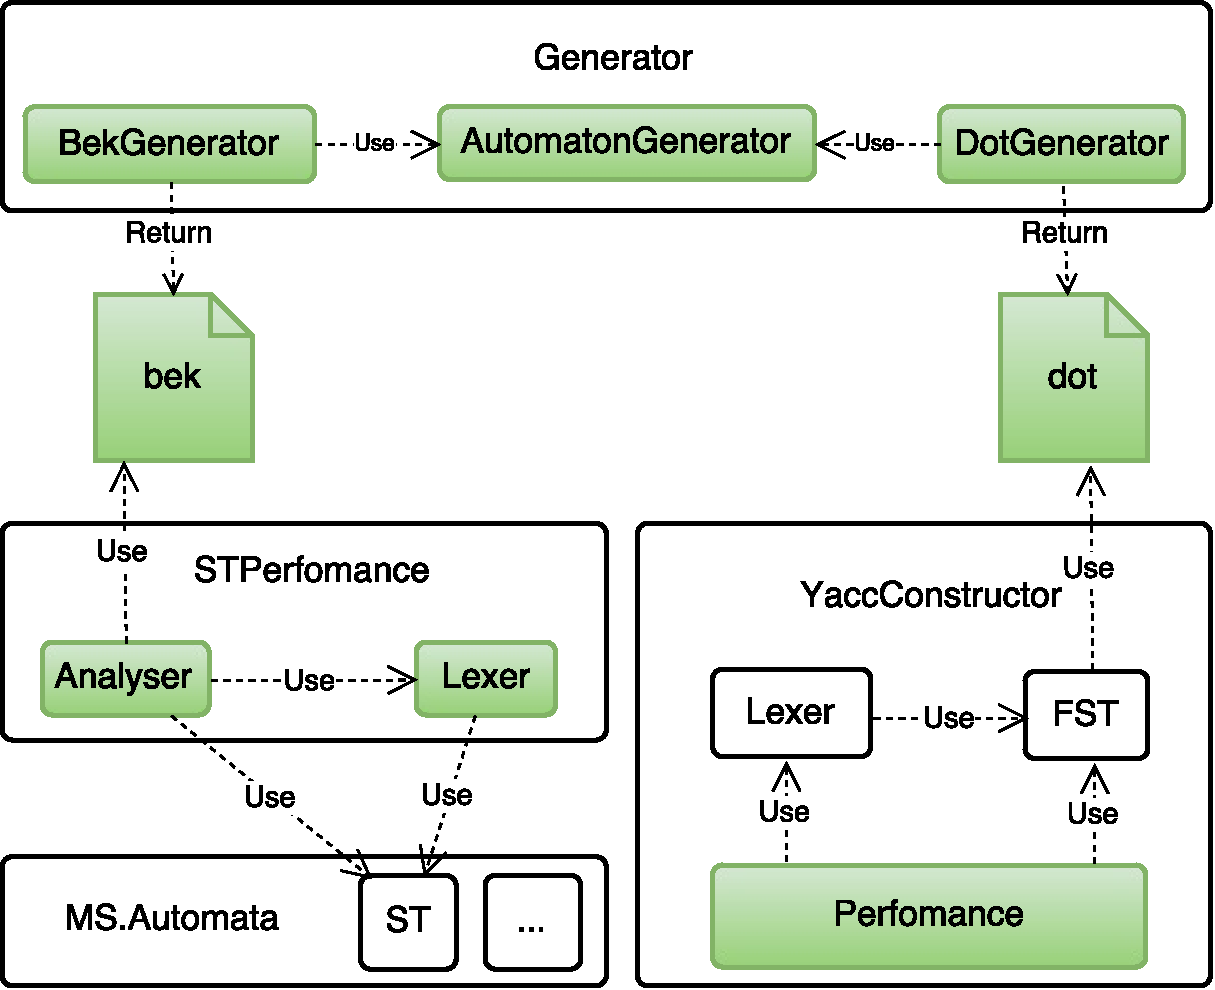
\includegraphics[width=\linewidth]{../pictures/YC.pdf}
        \caption{Архитектура среды для тестирования}
        \label{fig:toolStructure} 
    \end{center}
\end{figure}

% * <colored.lime@gmail.com> 16:40:16 25 May 2016 UTC+0300:
% косяк с графоном
Окружение состоит из:
\begin{itemize}
\item генератора конечных автоматов для создания на их основе эквивалентных преобразователей для инструмента YaccConstructor и библиотеки Microsoft.Automata;
\item генератора конечных преобразователей;
\item генератора символьных конечных преобразователей;
\item лексического анализатора в форме конечного преобразователя;
\item лексического анализатора в форме символьного конечного преобразователя;
\item модуля для анализа производительности операции композиции в проекте YaccConstructor;
\item модуля для анализа производительности операции композиции в библиотеке Microsoft.Automata.
\end{itemize}
Подробное описание компонентов приведено далее.

\subsection{Лексический анализатор}
Для сравнения времени работы операции композиции на символьных конечных преобразователях и конечных преобразователях было решено реализовать лексический анализатор арифметических выражений, аналогичный анализатору, который уже был интегрирован в проект YaccConstructor, так как язык арифметических выражений является достаточно показательным примером и включается практически в любой язык программирования.  Лексический анализатор может быть представлен в виде символьного конечного преобразователя и используется для анализа производительности библиотеки Microsoft.Automata. Реализация данного лексического анализатора выполнена на языке Bek.

\subsection{Генераторы преобразователей}
Генератор конечных автоматов (обозначен как AutomatonGenerator на рисунке~\ref{fig:toolStructure}) генерирует случайные конечные автоматы с указанным количеством дуг и вершин. Результат его работы --- файл с промежуточным представлением конечного автомата, который далее интерпретируется генераторами конечных преобразователей (обозначены как BekGenerator и DotGenerator на рисунке~\ref{fig:toolStructure}), которые на его основе строят программы, представляющие эквивалентные преобразователи, записанные на языках Bek и DOT соответственно. 

\subsection{Тестирование производительности композиции в проекте YaccConstructor на конечных преобразователях}
За тестирование производительности операции композиции на конечных преобразователях в проекте YaccConstructor отвечает модуль AbstractLexer.Interpreter.Perfomance (обозначен как Perfomance на рисунке~\ref{fig:toolStructure}). По dot-файлам лексического анализатора арифметических выражений и dot-файлам, сгенерированными модулем DotGenerator строятся конечные преобразователи. Затем производится композиция преобразователя, построенного по лексическому анализатору с каждым из тестовых преобразователей. Тест многократно повторяется и для каждого теста берется среднее значение затраченного времени.

\subsection{Тестирование производительности композиции в библиотеке Microsoft.Automata на символьных конечных преобразователях}
За тестирование производительности операции композиции на символьных конечных преобразователях в библиотеке Microsoft.Automata отвечает модуль PerfomanceTest (обозначен как STPerfomance на рисунке~\ref{fig:toolStructure}). По bek-файлам лексического анализатора арифметических выражений и bek-файлам, сгенерированными модулем BekGenerator строятся символьные конечные преобразователи. Затем производится композиция символьного преобразователя, построенного по лексическому анализатору с каждым из тестовых преобразователей. Тест многократно повторяется и для каждого теста берется среднее значение затраченного времени.

\subsection{Экспериментальное исследование}
С помощью описанного окружения был поставлен следующий эксперимент.

\begin{enumerate}
\item Сгенерированы пять конечных автоматов, характеристики которых указаны в таблице~\ref{table}.
\item По автоматам сгенерированы программы на языке DOT.
\item По автоматам сгенерированы программы на языке Bek.
\item Проведена композиция сгенерированных конечных преобразователей из dot-файлов с конечным преобразователем, представляющим лексический анализатор языка арифметических выражений из проекта YaccConstructor (операция повторялась 100 раз, в качестве результирующего значения взято среднее).
\item Проведена композиция сгенерированных символьных конечных преобразователей из bek-файлов с символьным конечным преобразователем, представляющим лексический анализатор языка арифметических выражений, аналогичный анализатору из YaccConstructor (операция повторялась 100 раз, в качестве результирующего значения взято среднее).
\end{enumerate}

В результате эксперимента получены данные, которые представлены на рисунке~\ref{graph1}.

\begin{figure}[H]
\begin{center}
\begin{tikzpicture}
\begin{axis}[
xtick=data,
legend pos = north west,
width=11.5cm,
xlabel = {Номер теста},
ylabel = {Время, мс}
]
\addplot coordinates {
(1,0.15) (2,0.39) (3,2.28) (4,5.02) (5,6.23)
};
\addplot coordinates {
(1,0.68) (2,4.82) (3,45.81) (4,167.91) (5,247.21)
};
\legend{конечный преобразователь, символьный преобразователь};
\end{axis}
\end{tikzpicture}
\end{center}

\caption{Результаты измерения скорости работы операции композиции на символьных преобразователях и конечных преобразователях}
\label{graph1}
\end{figure}

\begin{table}[H]
\begin{center}
\begin{tabular}{|c|c|c|}
\hline 
Тест & Ребра & Вершины\\  
\hline 
1 & 1 & 2 \\
2 & 6 & 5 \\
3 & 25 & 20 \\
4 & 50 & 5 \\
5 & 60 & 50 \\
\hline 
\end{tabular}
\caption{Размеры сгенерированных автоматов}
\label{table} 
\end{center}
\end{table} 

Эксперимент показал, что операция композиции над символьными конечными преобразователями в библиотеке Microsoft.Automata работает гораздо медленнее, чем операция композиции над конечными преобразователями в проекте YaccConstructor. В связи с этим было принято решение проанализировать производительность самой библиотеки. 

Анализ горячих точек показал, что при выполнении задач лексического анализа большую часть времени библиотека тратит на обращения к ядру библиотеки Z3. Поскольку в наших задачах отсутствует необходимость в использовании Z3, было решено в качестве эксперимента отключить некоторые затратные проверки условий, чтобы сократить количество обращений к ядру. Эксперимент показал, что таким образом можно как минимум увеличить производительность операции композиции на 20\% на некоторых тестах (время работы операции композиции на модифицированной библиотеке отражено на рисунке~\ref{graph2}), что показывает, что адаптация библиотеки к нашей задаче может способствовать увеличению производительности, но этого недостаточно для получения оптимальных результатов.


\begin{figure}[H]
\begin{center}
\begin{tikzpicture}
\begin{axis}[
xtick=data,
legend pos = north west,
width=11.5cm,
xlabel = {Номер теста},
ylabel = {Время, мс}
]
\addplot coordinates {
(1,0.68) (2,4.82) (3,45.81) (4,167.91) (5,247.21)
};
\addplot coordinates {
(1,0.54) (2,3.6) (3,35.08) (4,128.07) (5,190.76)
};
\legend{библиотека, модифицированная библиотека};
\end{axis}
\end{tikzpicture}
\end{center}
\caption{Результаты измерения скорости работы операции композиции на символьных преобразователях с модифицированной и обычной версиями библиотеки}
\label{graph2}
\end{figure}

В результате экспериментов были сделаны выводы, что библиотека Microsoft.Automata, разработанная для решения задач из области формальной верификации, недостаточно производительна для лексического анализа. Большое количество обращений к ядру Z3 перекрывает все достоинства, приобретаемые от использования оптимального формализма и структур данных. Таким образом, применение библиотеки Microsoft.Automata в инструменте YaccConstructor для лексического анализа в настоящий момент неоптимально. 
Использование же символьных конечный преобразователей для лексического анализа все еще выглядит перспективным и подлежит дальнейшему исследованию.

% У заключения нет номера главы
\section*{Заключение}
В рамках выполнения данной работы были получены следующие результаты.
\begin{itemize}
\item Исследованы возможности библиотеки Microsoft.Automata.
\item Проведено сравнение производительности алгоритма операции композиции над символьными конечными преобразователями в библиотеке с производительностью операции композиции над конечными преобразователями в проекте YaccConstructor.
\item На основании полученных результатов сделаны выводы о необходимости написания собственной реализации символьного конечного преобразователя.
\item Результаты работы представлены на конференции «Современные технологии в теории и практике программирования», тезисы опубликованы в сборнике материалов конференции.
\end{itemize}

Код генераторов автоматов и преобразователей, а также код, тестирующий производительность символьных преобразователей в библиотеке Microsoft.Automata можно найти на сайте \url{https://github.com/GuminEgor/Automata}. Код, тестирующий производительность конечных преобразователей в проекте  YaccConstructor можно найти на сайте \url{https://github.com/GuminEgor/YaccConstructor}. В указанных репозиториях автор принимал участие под учетной записью GuminEgor.

В дальнейшем необходима реализация собственной версии символьного конечного преобразователя, адаптированного под задачи лексического анализа, тестирование его производительности и, в случае удовлетворительных результатов, его интеграция в проект YaccConstructor.



\setmonofont[Mapping=tex-text]{CMU Typewriter Text}
\bibliographystyle{ugost2008ls}
\bibliography{diploma.bib}
\end{document}
